\section{Absolute Value Inequalities}
\textbf{Example.} What x-values satisfy $|x|<$5? \\
\textbf{Solution.} We can solve this problem by using a number line. We know that the distance between x and 0 is less than 5. So, the x-values that satisfy the inequality are somewhere between -5 to 5. \\
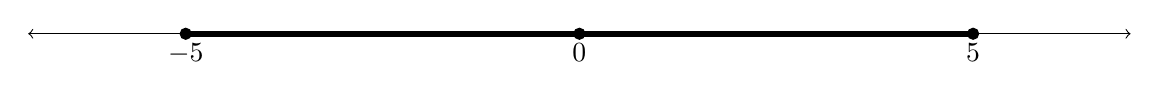
\begin{tikzpicture}
    % Draw the number line
    \draw[<->] (-7,0) -- (7,0);

    % Mark 0
    \draw[fill=black] (0,0) circle (2pt) node[below] {$0$};

    % Mark -5
    \draw[fill=black] (-5,0) circle (2pt) node[below] {$-5$};

    % Mark 5
    \draw[fill=black] (5,0) circle (2pt) node[below] {$5$};

    % Bold line between -5 and 5
    \draw[line width=2pt] (-5,0) -- (5,0);
\end{tikzpicture}
We can express this inequality without using absolute value. We know that $|x|<$5 is equivalent to $-5<x<5$. Because $x$ is somewhere between -5 and 5. Therefore the solution is $-5<x<5$. Or as an interval notation: $(-5,5)$.
\\
\vspace{4pt}
\textbf{Example.} What x-values satisfy $|x|\geq5$? \\
Since $|x|$ has to be greater than or equal to 5, $|x|$ has to be bigger then 5 and -5, since it can be both positive and negative. So, the x-values that satisfy the inequality are somewhere less than -5 or greater than 5. \\
\\
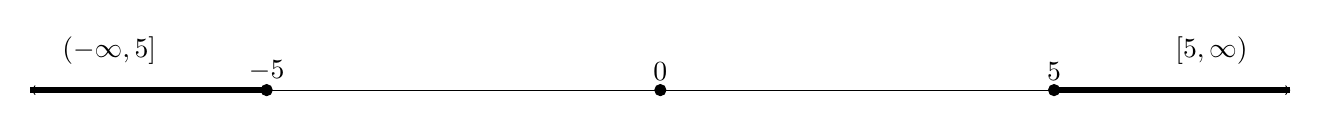
\begin{tikzpicture}
    % Draw the number line
    \draw[<->] (-8,0) -- (8,0);

    % Mark 0, 5, and -5 with filled circles
    \draw[fill=black] (0,0) circle (2pt) node[above] {$0$};
    \draw[fill=black] (5,0) circle (2pt) node[above] {$5$};
    \draw[fill=black] (-5,0) circle (2pt) node[above] {$-5$};

    % Mark the regions to be emphasized with bold lines
    \draw[line width=2pt] (-8,0) -- (-5,0);
    \draw[line width=2pt] (5,0) -- (8,0);

    % Label the emphasized regions
    \node at (-7,0.5) {$(-\infty, 5]$};
    \node at (7,0.5) {$[5, \infty)$};
\end{tikzpicture}

So, $x\leq-5$ or $x\geq5$. Or as an interval notation: $(-\infty, -5]\cup[5, \infty)$.

\textbf{Example.} Solve $|3-2t|<4$. 

Since $|3-2t|$ has to be less than 4 OR bigger -4 we can represent it in a numberline.  \\
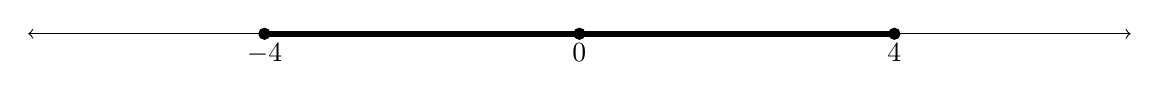
\begin{tikzpicture}
    % Draw the number line
    \draw[<->] (-7,0) -- (7,0);

    % Mark 0
    \draw[fill=black] (0,0) circle (2pt) node[below] {$0$};

    % Mark -5
    \draw[fill=black] (-4,0) circle (2pt) node[below] {$-4$};

    % Mark 5
    \draw[fill=black] (4,0) circle (2pt) node[below] {$4$};

    % Bold line between -5 and 5
    \draw[line width=2pt] (-4,0) -- (4,0);
\end{tikzpicture}

Therefore, we can just have two different equations: 
\begin{align*}
    3-2t<4 \\
    3-2t>-4
\end{align*}
Solving the first equation:
\begin{align*}
    3-2t<4 \\
    -2t<1 \\
    t>-\frac{1}{2}
\end{align*}
Solving the second equation:
\begin{align*}
    3-2t>-4 \\
    -2t>-7 \\
    t<\frac{7}{2}
\end{align*}

In the numberline we can see that the solution is $-\frac{1}{2}<t<\frac{7}{2}$. \\
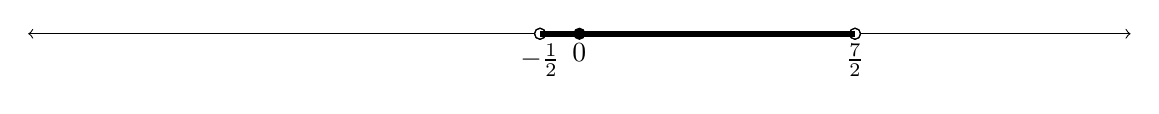
\begin{tikzpicture}
    % Draw the number line
    \draw[<->] (-7,0) -- (7,0);

    % Mark 0
    \draw[fill=black] (0,0) circle (2pt) node[below] {$0$};

    % Mark -1/2 with a hole
    \draw[fill=white] (-1/2,0) circle (2pt) node[below] {$-\frac{1}{2}$};
    \draw (-1/2,0) circle (2pt); % Draw a hole in the circle

    % Mark 7/2 with a hole
    \draw[fill=white] (7/2,0) circle (2pt) node[below] {$\frac{7}{2}$};
    \draw (7/2,0) circle (2pt); % Draw a hole in the circle

    % Bold line between -1/2 and 7/2
    \draw[line width=2pt] (-1/2,0) -- (7/2,0);
\end{tikzpicture}

Or as an interval notation: $(-\frac{1}{2}, \frac{7}{2})$.

Notice that the solution cannot include $-\frac{1}{2}$ and $\frac{7}{2}$ because $|3-2t|$ cannot be equal to 4.